\section{\textbf{Experiment Setup and Observations}}

The set-up is as follows (Figure~\ref{fig:setup}):

\begin{figure}
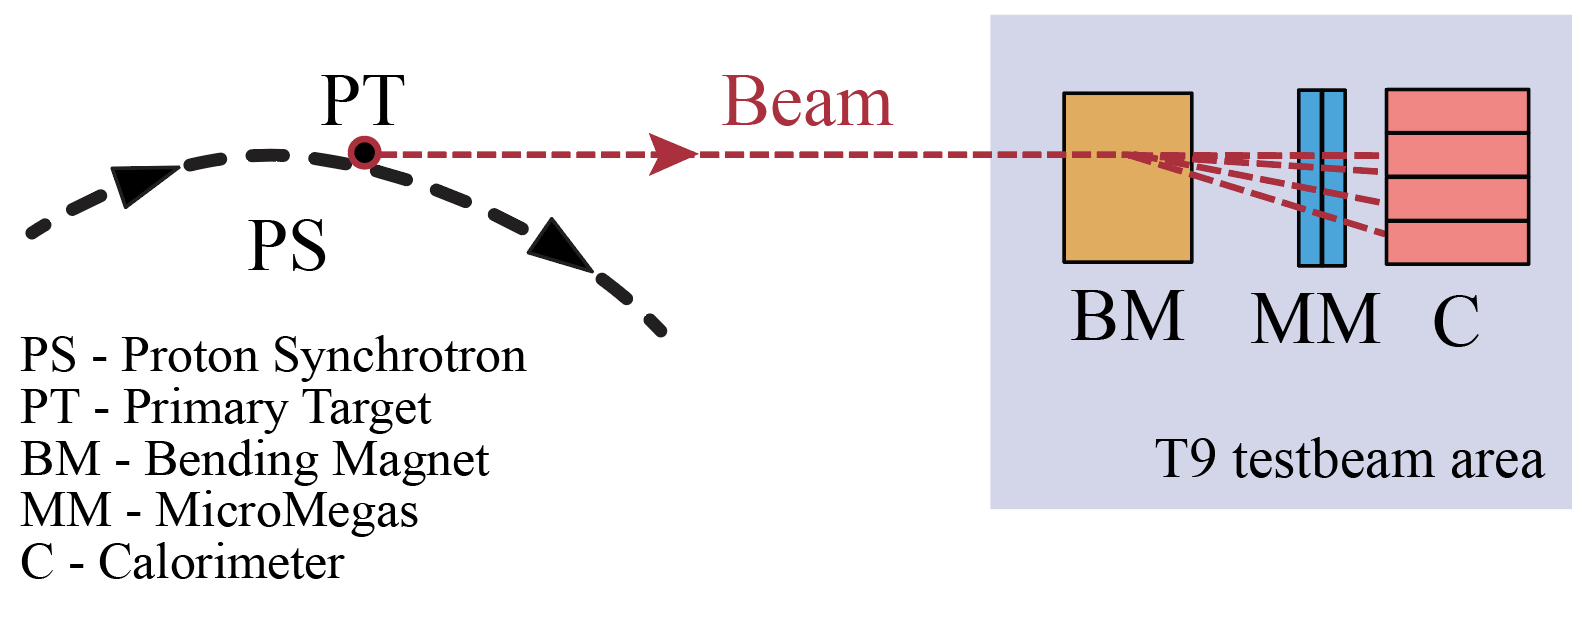
\includegraphics[width=\textwidth]{Sections/Diagrams/diagram.png}
\centering
\caption{Experimental setup diagram illustrating }
\label{fig:setup}
\end{figure}

\begin{enumerate}
    \item Standard set up consisting of the Proton Synchrotron ($PS$) and Primary Target ($PT$), where the beam generated can be positively or negatively charged.
    %\item A Collimator ($CO$) is used to control the momentum acceptance for each tested beam energy and beam divergence, such that only protons travelling within a circular cross-sectional area with diameter of $2\, cm$ are accepted. 
    \item In the test beam area, a Bending Magnet ($BM$) is placed in the beam's path. Each type of particles contained in the beam are diverged to varying degrees according to their charge and mass. The magnetic field value will be set to a constant.
    \item Two MicroMegas detectors ($MM$) of dimension 40x40cm are stacked such that their axes are perpendicularly aligned. This tracks the position of the diverged particles incident on the 2D plane perpendicular to the original beam. 
    \item 16 Lead Crystal Calorimeters ($C$) are arranged in a 4x4 square. This covers an area of 40x40cm, thus sufficiently capturing the energy of all particles passing through $MM$.
\end{enumerate}


Our experiment aims to compare the musical notes for different types of beams, for varying magnetic field, and for different ways of calculating the frequency or the loudness of the note. Table 1 can be updated with the results of the experiment, which will then be analysed to find correlations and causations.

\begin{table}[h!]
\centering
\begin{tabular}{||c c c||} 
 \hline
 Magnetic Field Intensity & Beam Dispersion & Frequency of Major Note\\ [0.5ex] 
 \hline\hline
 ... & ... & ... \\ 
 ... & ... & ... \\
 ... & ... & ... \\
 ... & ... & ... \\
 ... & ... & ... \\ [1ex] 
 \hline
\end{tabular}
\caption{Observation Table}
\label{table:1}
\end{table}